\documentclass[10pt]{article}

\usepackage{amssymb,amsmath,amsthm}
\usepackage{bm}
\usepackage{graphicx,subcaption,float}
\usepackage[letterpaper, margin=0.5in]{geometry}

\newtheorem{definition}{Definition}
\newtheorem{theorem}{Theorem}
\newtheorem{lemma}{Lemma}
\newtheorem{remark}{Remark}

\newcommand{\norm}[1]{\ensuremath{\left\| #1 \right\|}}
\newcommand{\fnorm}[1]{\ensuremath{\left\| #1 \right\|_\mathrm{F}}}
\newcommand{\tr}[1]{\ensuremath{\mathrm{tr}\left( #1 \right)}}
\newcommand{\etr}[1]{\ensuremath{\mathrm{etr}\left\{ #1 \right\}}}
\newcommand{\expect}[1]{\ensuremath{\mathrm{E}\left[ #1 \right]}}
\newcommand{\expectbar}[1]{\ensuremath{\bar{\mathrm{E}}\left[ #1 \right]}}
\newcommand{\SO}{\ensuremath{\mathrm{SO(3)}}}
\newcommand{\real}[1]{\ensuremath{\mathbb{R}^{ #1 }}}
\newcommand{\diff}[1]{\ensuremath{\mathrm{d} #1}}
\newcommand{\expb}[1]{\ensuremath{\mathrm{exp}\left\{#1\right\}}}

\title{\vspace{-4ex}\textbf{Analytical Uncertainty Propagation of Matrix Fisher-Gaussian Distribution\vspace{-4ex}}}
\date{}

\graphicspath{{./Figs/}}

\begin{document}

\maketitle

Consider the following model
\begin{gather*}
	R_{k+1} = R_k\exp(\hat{x}_k), \qquad R'_{k+1} = R_k + R_k\hat{x}_k \\
	x_{k+1} = x_k.
\end{gather*}
Suppose at $t=t_k$, $(R_k,x_k)$ follows a matrix Fisher-Gaussian distribution with parameters $(\mu_k,\Sigma_k,P_k,U_k,S_k,V_k)$, where $\mu_k = 0$, $P_k = 0$, $\Sigma_k = 0.1^2I_{3\times 3}$, $S_k = \mathrm{diag}(200,0,0)$, $U_k=V_k=I_{3\times 3}$.

Let us draw 1 million samples from $\mathcal{MG}(\mu_k,\Sigma_k,P_k,U_k,S_k,V_k)$, and propagate them through the kinematic equations.
Define the following
\begin{gather}
	U_{k+1}\frac{\partial c(S_{k+1})}{\partial S_{k+1}}V_{k+1}^T = \expectbar{R_{k+1}}, \qquad v_{R_{k+1}} = (U_{k+1}^TR_{k+1}V_{k+1}S_{k+1} - S_{k+1}V_{k+1}^TR_{k+1}U_{k+1})^\vee \\
	v'_{R_{k+1}} = (U_k^TR'_{k+1}V_kS_k - S_kV_k^TR'^T_{k+1}U_k)^\vee.
\end{gather}

The following figures are $x_{k+1}$ against $\nu_{R_{k+1}}$ and $\nu'_{R_{k+1}}$.

\begin{figure}[H]
	\centering
	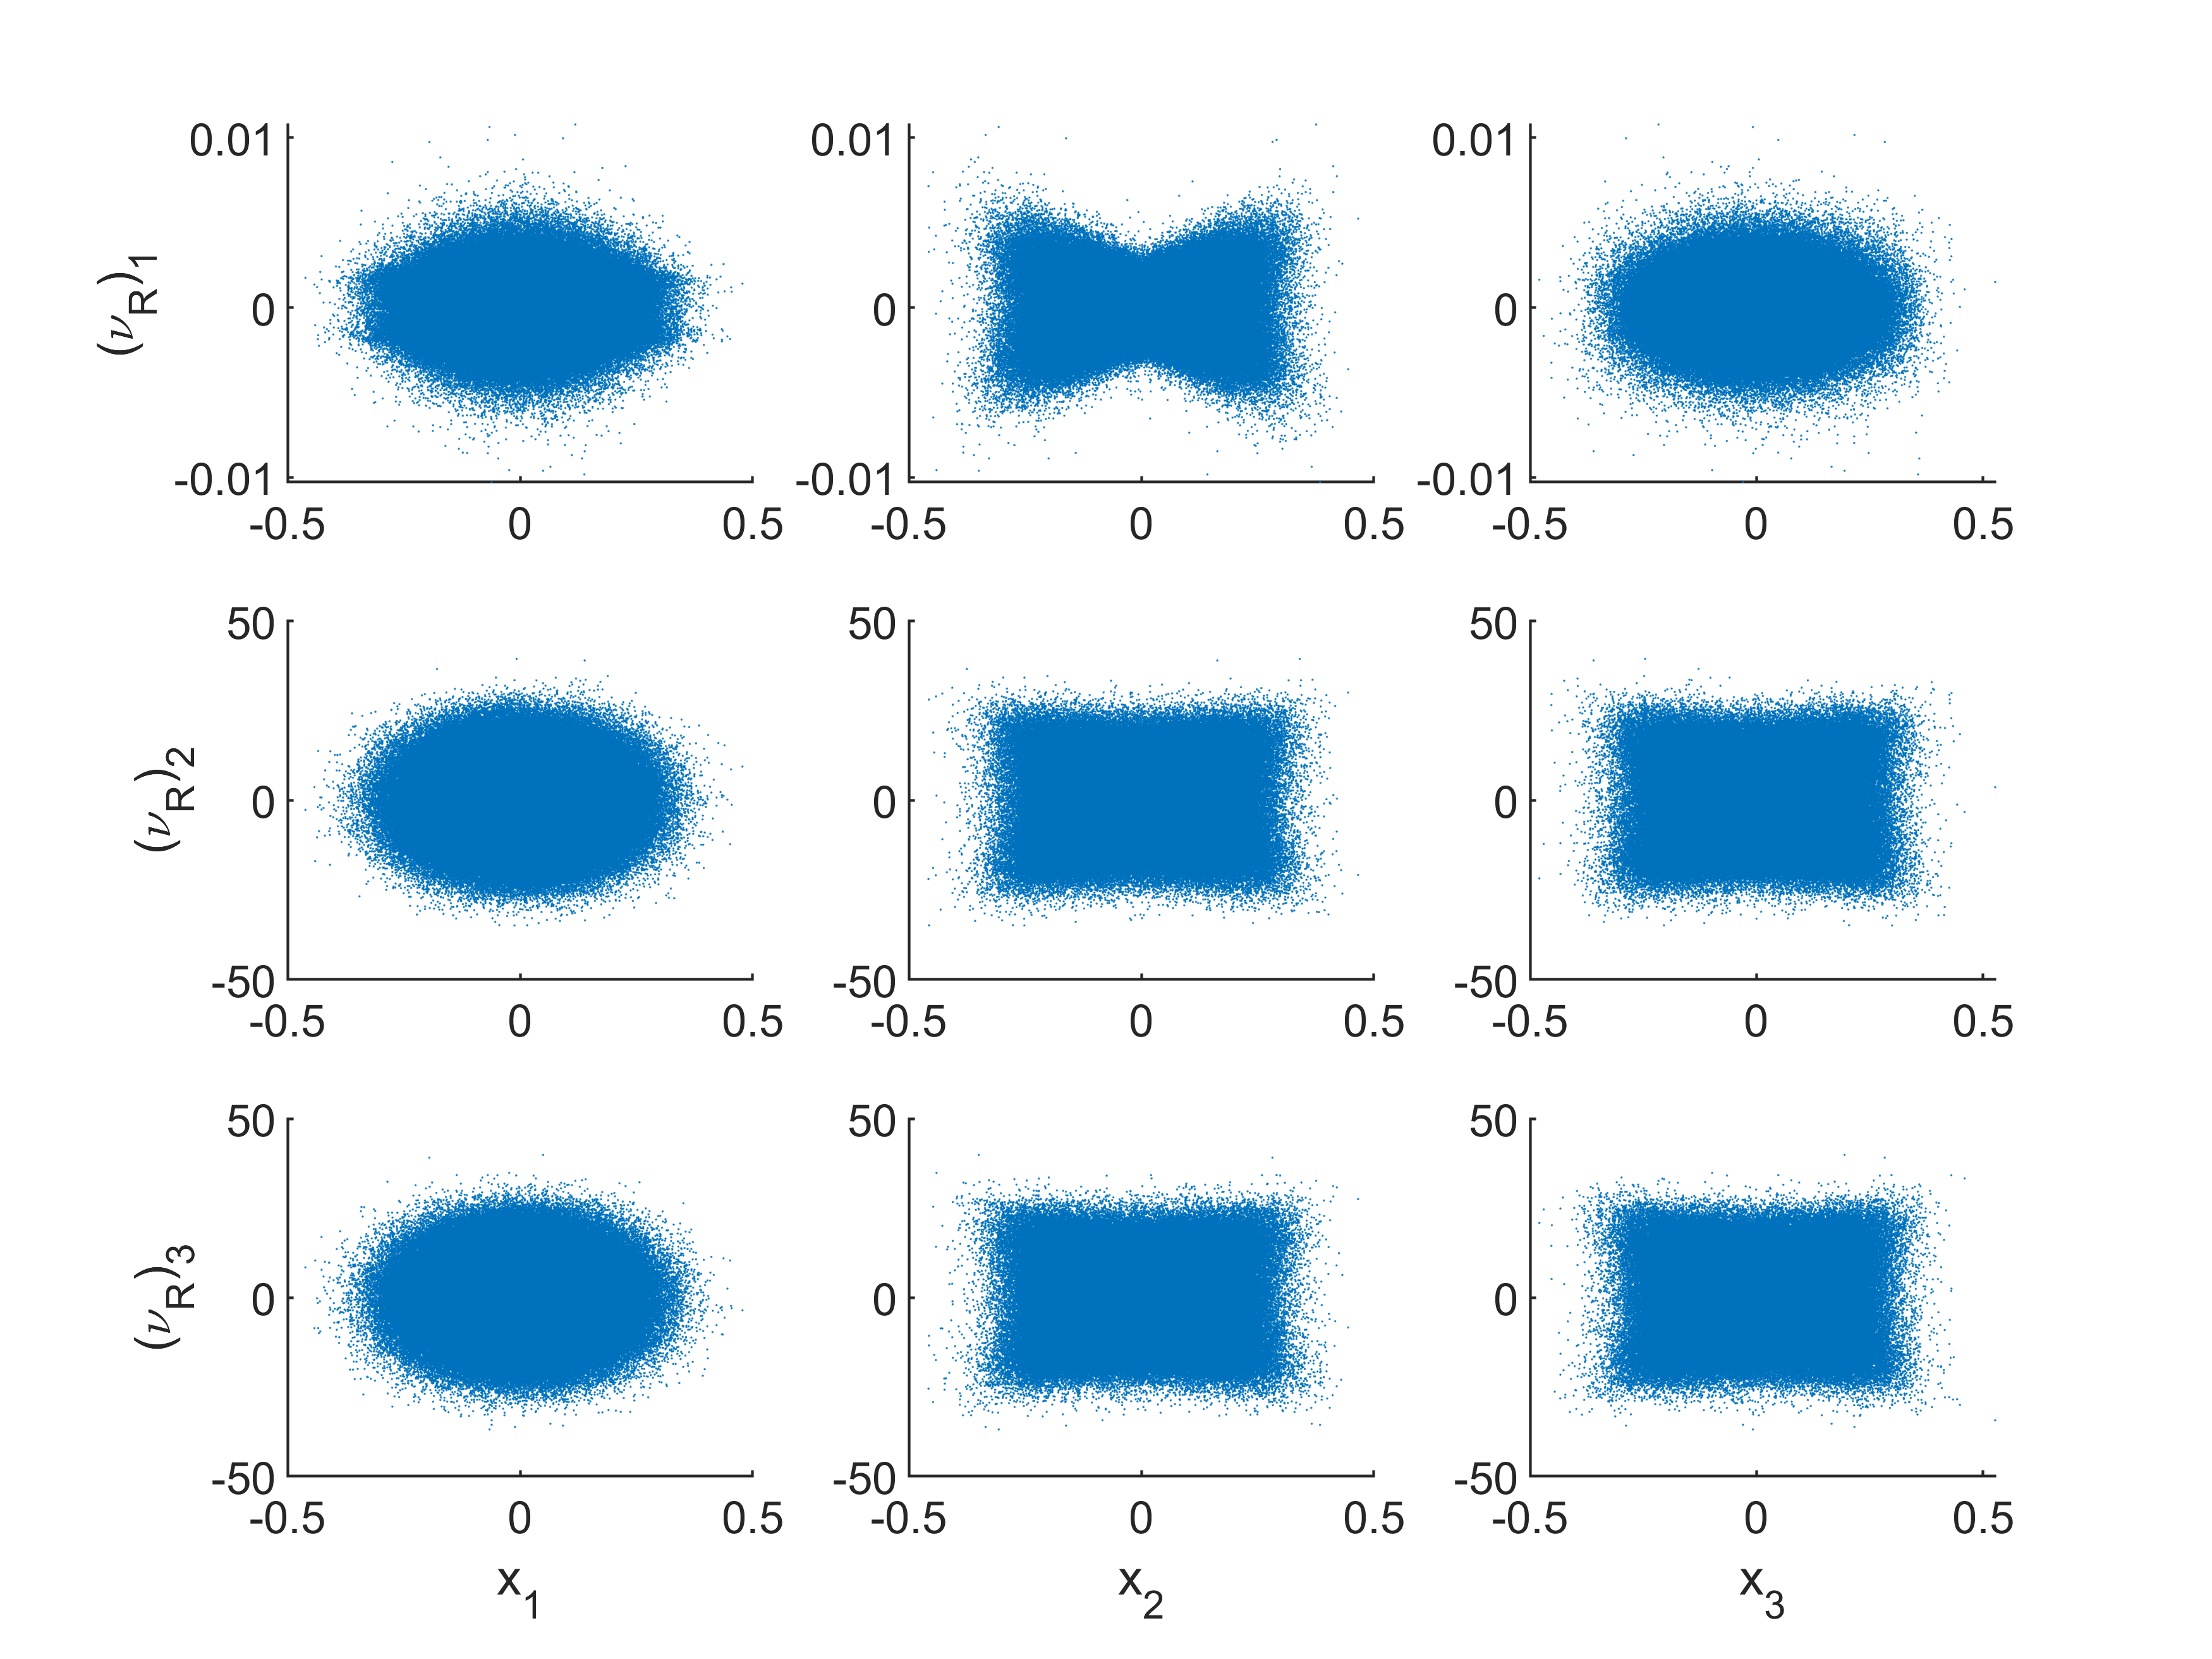
\includegraphics{xvR}
\end{figure}

\begin{figure}[H]
	\centering
	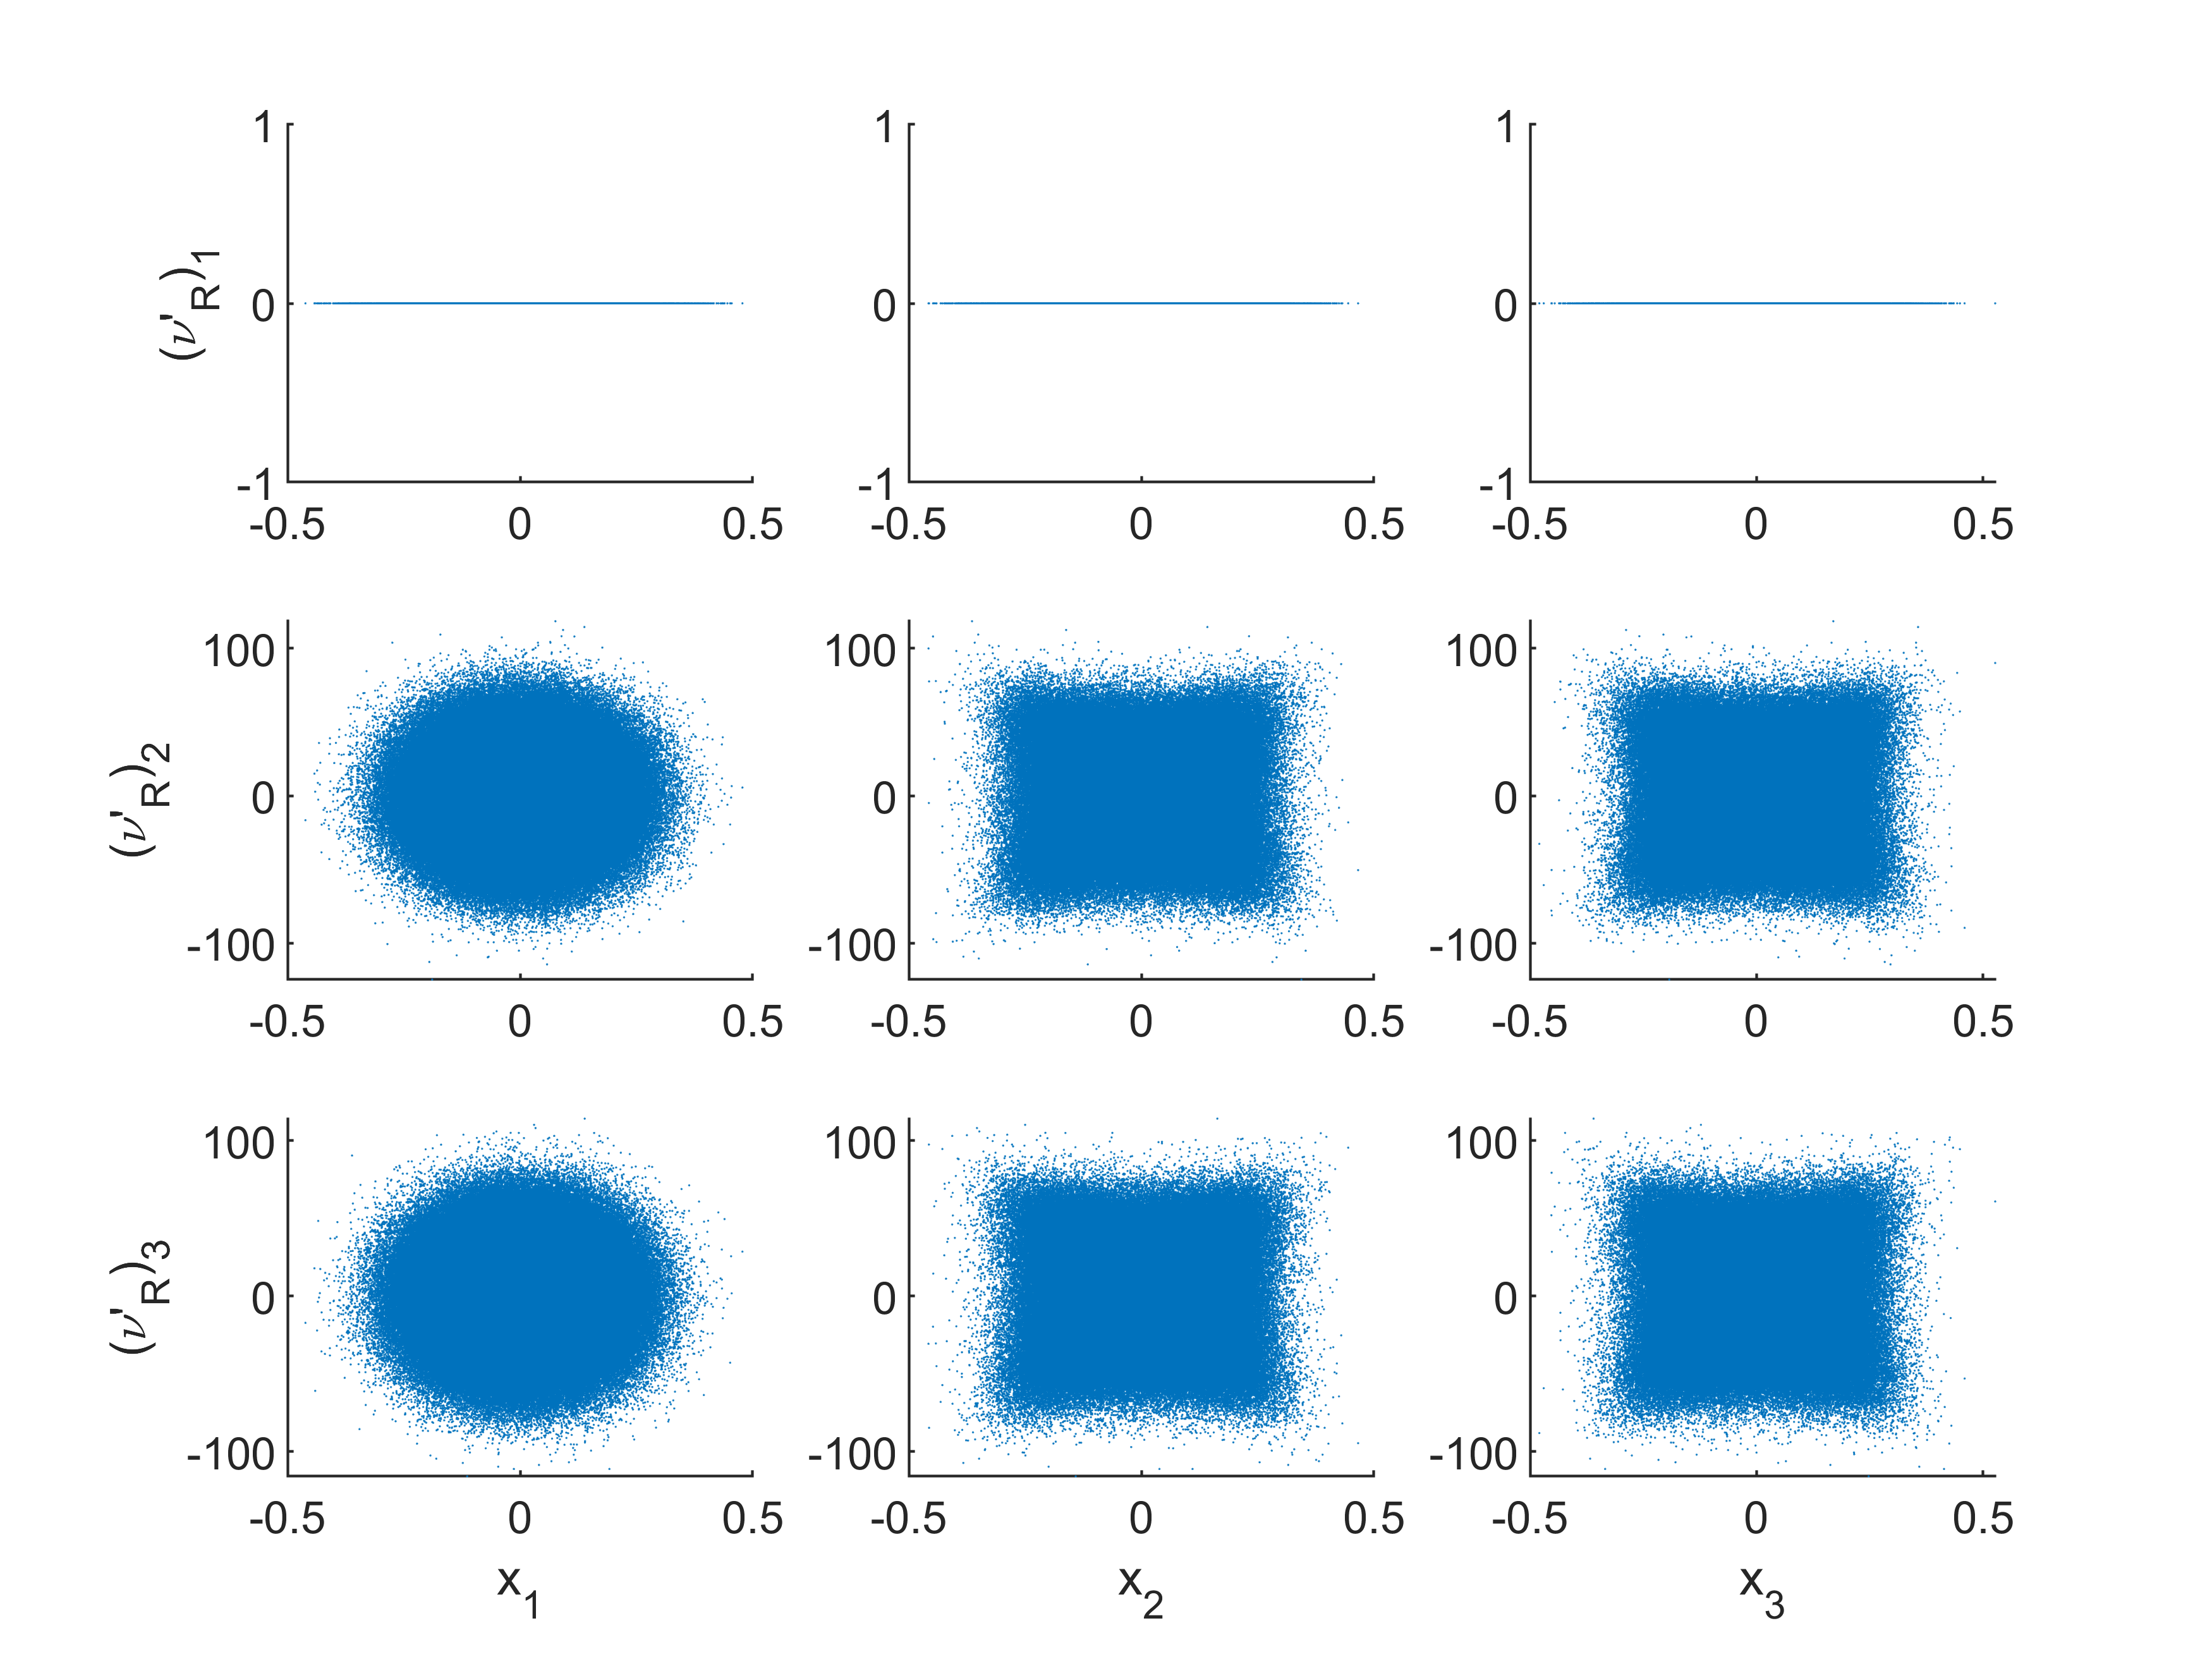
\includegraphics{xvRprime}
\end{figure}

The observation is clear, the correlation between $x_{k+1}$ and $\nu_{R_{k+1}}$ or $\nu'_{R_{k+1}}$ is approximately zero.
The major difference between $\nu_{R_{k+1}}$ or $\nu'_{R_{k+1}}$ is that $(s_1)_{k+1}$ is much smaller than $(s_1)_k$ since it incorporates the uncertainty in $x_k$ without the $h^2$ coefficient.
Also, $U_{k+1}V_{k+1}^T$ is an arbitrary rotation about the body fixed $e_1$-axis from $I_{3\times 3}$.

Now define $\delta\theta_{k+1} = \log((U_{k+1}V_{k+1}^T)^{-1}R_{k+1})^\vee$, the following figure is $x_{k+1}$ against $\delta\theta_{k+1}$.

\begin{figure}[H]
	\centering
	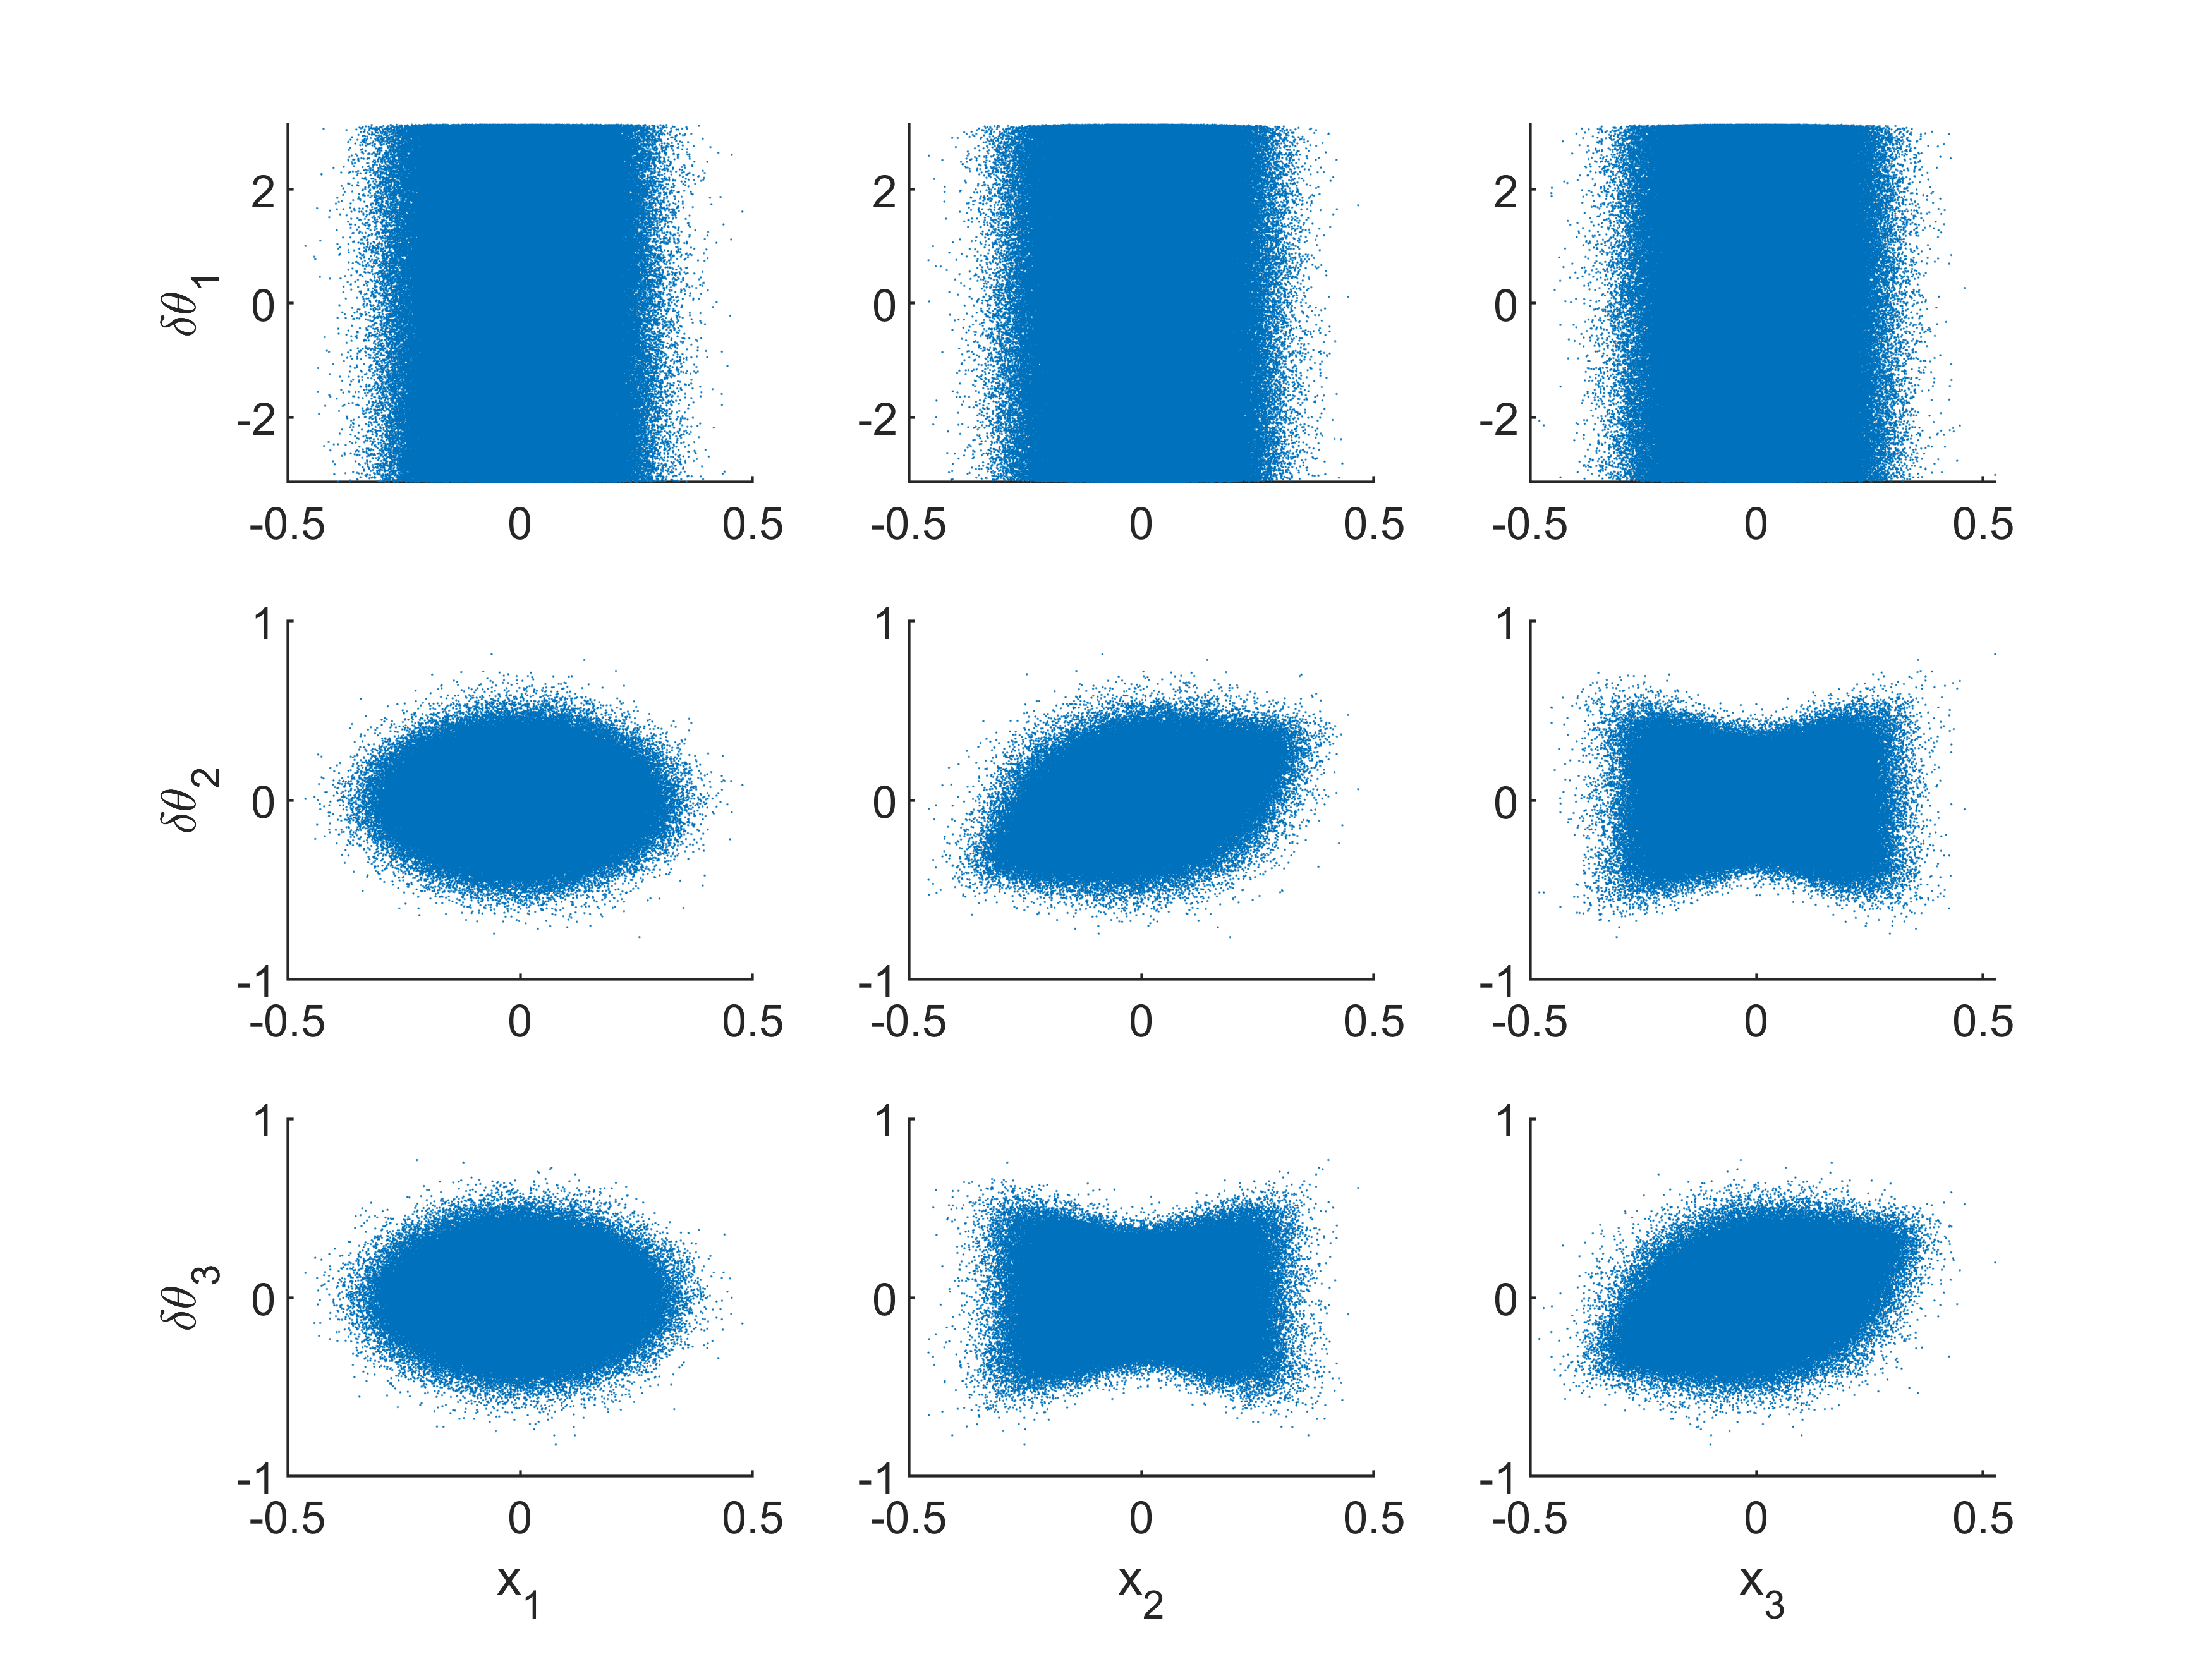
\includegraphics{xtheta}
\end{figure}

It is clearly seen $x_2$, $\delta\theta_2$ and $x_3$, $\delta\theta_3$ are correlated.

\end{document}

